% ----------------------------------------------------------------------
% ----------------------------------------------------------------------
\section*{Prinzip}
Backpropagation ist ein \emph{Gradientenabstiegsverfahren} und die Erweiterung der Delta-Regel auf mehrere trainierbare Gewichtsschichten, weil bei mehrstufigen Netzen keine erwünschte Ausgabe als Lerneingabe (teaching input) für die Zellen \emph{innerer Ebenen} vorhanden ist.

Wenn man den Fehler eines neuronalen Netzes als Funktion der Gewichte des Netzwerks graphisch aufträgt, erhält man eine Fehlerfläche, welche sich im zweidimensionalen Fall anschaulich graphisch darstellen lässt.

\begin{figure}[ht!] \centering 
	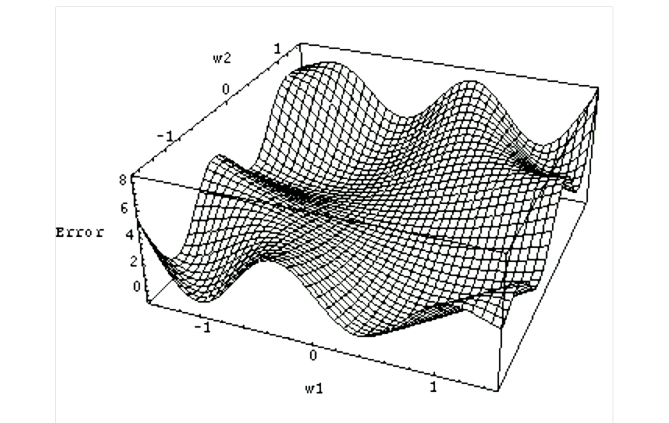
\includegraphics[width=\linewidth]{figures/ch03_fehlerflaeche.pdf}
	\caption{Fehlerfunktion $Err(w_1, w_2)$ grafisch aufgetragen.}
	\label{fig:ch03_fehlerflaeche}
\end{figure}

Abbildung \ref{fig:ch03_fehlerflaeche} zeigt die Fehlerfunktion $Err(w_1, w_2)$. Bei $n$ Gewichten gilt allgemein:
\[
	Err(\vec{w}) = Err(w_1, \ldots, w_n)
\]
Diese Fehlerfunktion gibt den Fehler an, den das Netz bei gegebenen Gewichten $w_1, \ldots, w_n$ über alle Trainingsmuster aufsummiert besitzt.

Mit einem Gradientenverfahren, d.h. der Methode des steilsten Abstiegs, wird nun versucht, möglichst schnell ein globales Minimum der Fehlerfunktion zu finden, d.h. eine Konfiguration der Gewichte, bei der die Fehlersumme über alle Trainingsmuster minimal ist.



% ----------------------------------------------------------------------
% ----------------------------------------------------------------------
\section*{Gradientenverfahren}
Alle Gradientenverfahren (engl. gradient decent) berechnen den Gradienten einer Zielfunktion, hier der Fehlerfunktion, und steigen entweder orthogonal zum Gradienten nach oben, bis ein Maximum erreicht ist oder nach unten, bis ein Minimum erreicht ist.
Hier wird versucht, durch Änderung der Gewichte den Fehler zu minimieren, indem eine Änderung aller Gewichte um einen Bruchteil des negativen Gradienten der Fehlerfunktion vorgenommen wird.
Es gilt der Zusammenhang, welcher schon im vorherigen Abschnitt bei den Fehlerfunktionen behandelt wurde:
\begin{align*}
	\Delta w &= - \eta \nabla Err(w) \\
	\Delta w_{i,\Omega} &= - \eta \frac{\partial Err(w)}{\partial w_{i,\Omega}}
\end{align*}

\begin{figure}[ht!] \centering 
	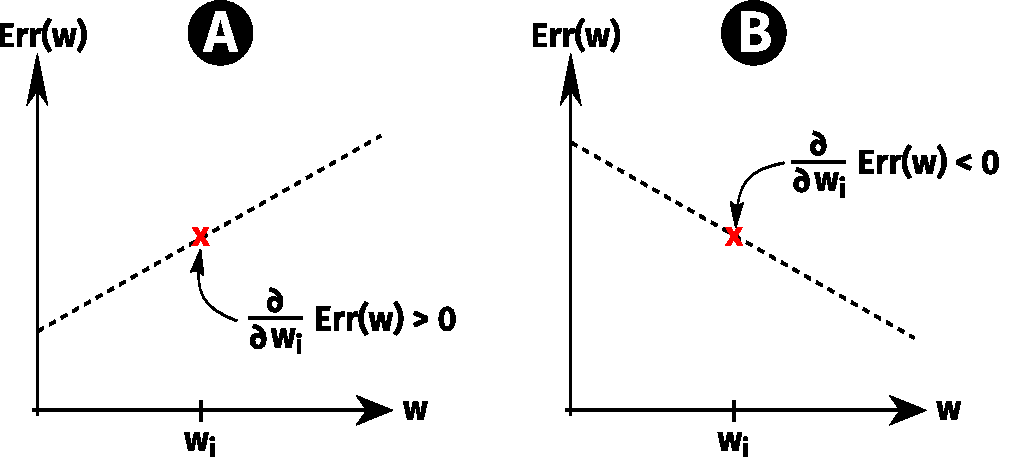
\includegraphics[width=\linewidth]{figures/ch03_gradient-decent.pdf}
	\caption{Gradientenabstieg grafisch dargestellt. Im Fall \emph{A} ist die Steigung der Fehlerfunktion beim Gewicht $w_i$ positiv, das Gewicht muss demnach verkleinert werden, damit der Fehler kleiner wird. Im Fall \emph{B} hingegen ist die Steigung bei $w_i$ negativ, das Gewicht muss dementsprechend erhöht werden, um die Kosten zu reduzieren. Dies ist der Grund für das Minuszeichen in der Gleichung.}
	\label{fig:ch03_fehlerflaeche}
\end{figure}

Auch beim Gradientenabstiegsverfahren unterscheidet man zwischen online und offline Verfahren: 
\begin{itemize}
	\item \emph{Stochastic Gradient Descent} - Die Anpassung der Gewichte findet nach jedem Trainingsbeispiel statt. Daher ist dieses Verfahren robuster gegen nicht-konvexe Fehlerfunktionen. 
	\item \emph{Batch Gradient Descent} - Hier werden die Änderungen der Gewichte über eine Epoche hinweg aufaddiert und erst anschließend auf die Gewichte angewandt.
\end{itemize}


% ----------------------------------------------------------------------
% ----------------------------------------------------------------------
\section*{Verallgemeinerung der Delta-Regel}
Zur Veranschaulichung der verallgemeinerten Delta-Regel, genannt \emph{Backpropagation of Error} oder kurz \emph{Backpropagation} dient das in Abbildung \ref{fig:ch03_fehlerflaeche} dargestellte Multi-Layer-Perzeptron (MLP).
Formal ergibt sich daraus folgender Zusammenhang:
\begin{align*}
	\Delta w_{k,h} &= \eta \cdot o_k \cdot \delta_h \\
	&\text{mit} \\
	\delta_h &=
	\begin{cases}
		f'_{act}(net_h) \cdot (t_h - y_h) 
		\quad &\text{wenn h außen} \\
		f'_{act}(net_h) \cdot \sum_{l \in L} (\delta_l \cdot w_{h,l})
		\quad &\text{wenn h innen}
	\end{cases}
\end{align*}

\begin{figure}[ht!] \centering 
	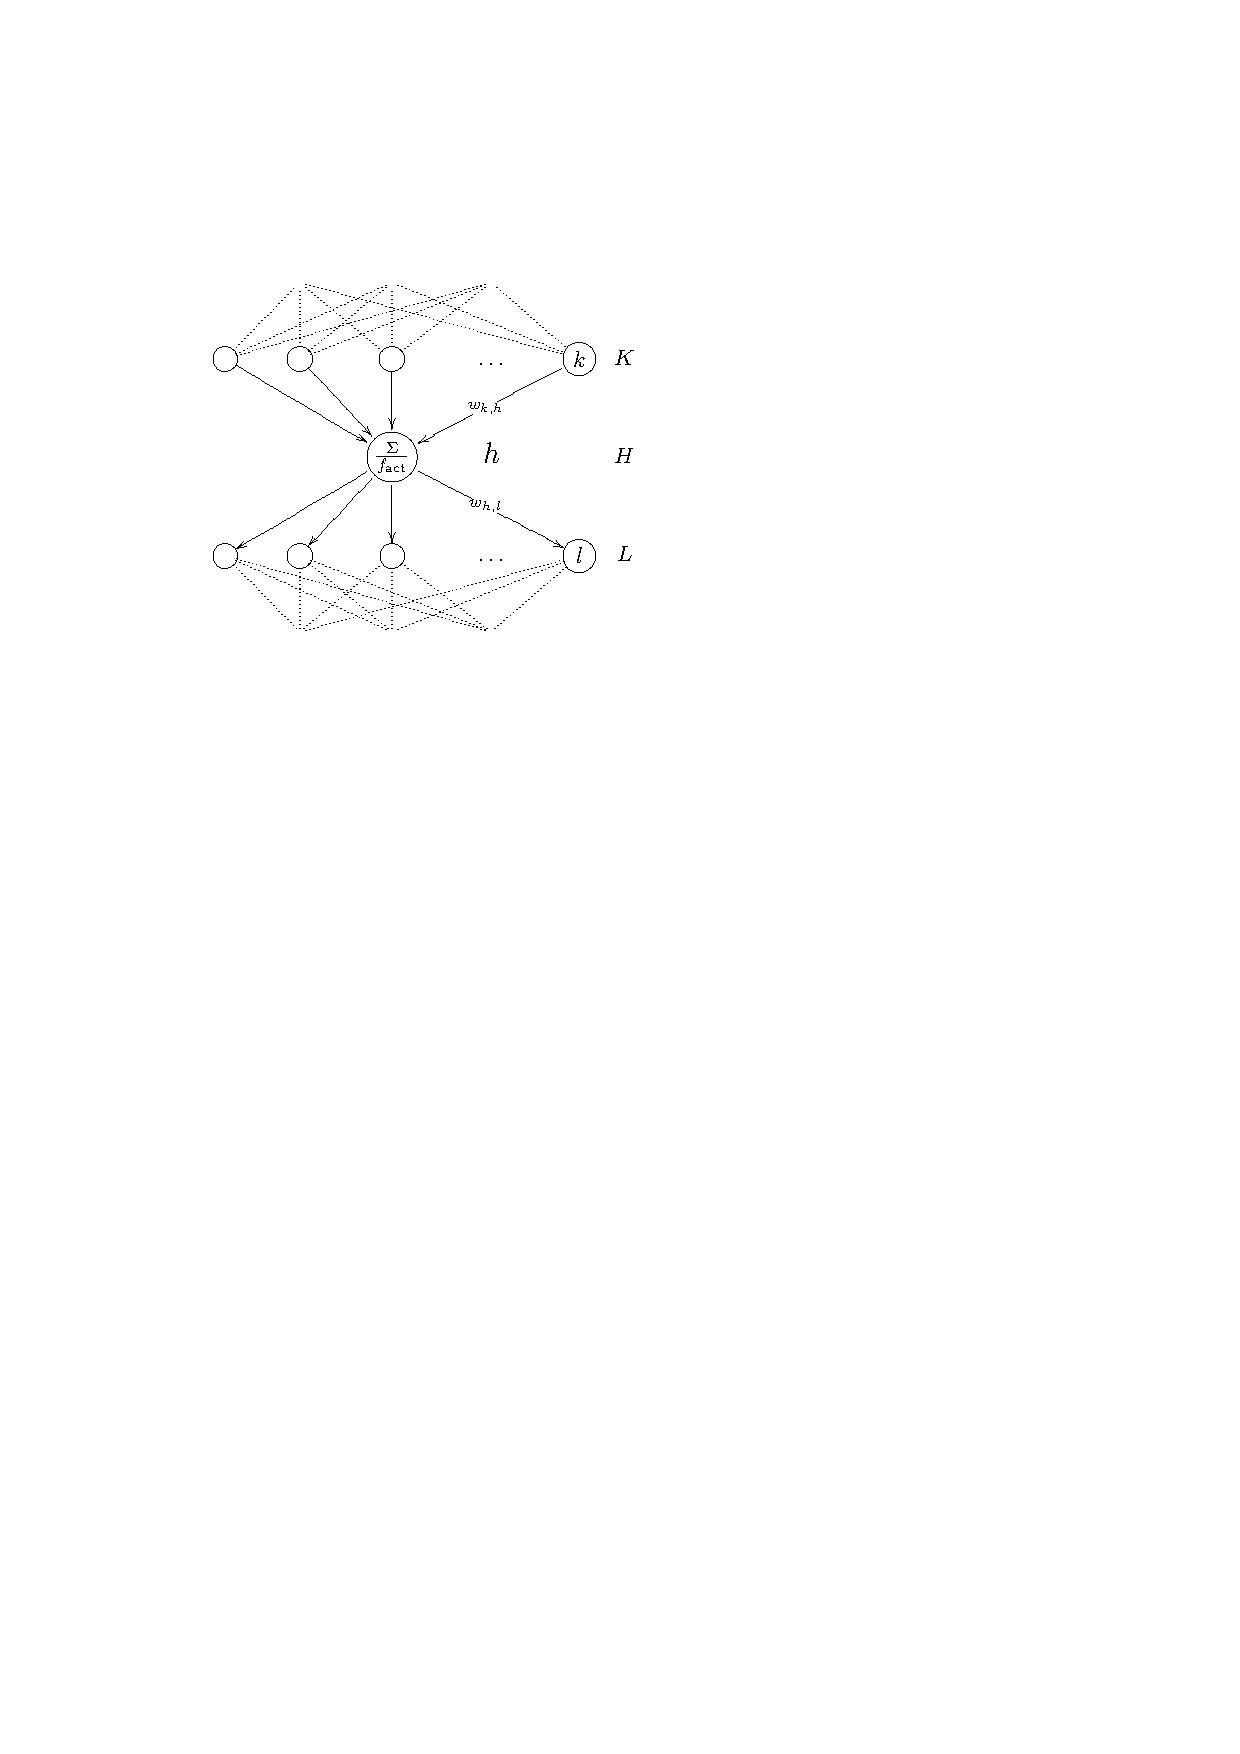
\includegraphics[width=\linewidth]{figures/ch03_mlp-backpropagation.pdf}
	\caption{Diese Abbildung zeigt die Lage des in der Formel für Backpropagation betrachteten Neurons $h$ in einer Hiddenschicht $H$. Die Vorgängerschicht ist $K$, die nachfolgende Schicht $L$. Wichtig hierbei: $L$ ist \emph{nicht} die Ausgabeschicht, sonst würde für $h$ die einfache Delta-Regel gelten.}
	\label{fig:ch03_fehlerflaeche}
\end{figure}



% ----------------------------------------------------------------------
% ----------------------------------------------------------------------
\section*{Aktivierungsfunktionen für Backpropagation}
Aus der Formel für Backpropagation geht hervor, dass die Aktivierungsfunktion semilinear, d.h. monoton und differenzierbar, sein muss. Darüber hinaus muss gelten:
\[
	f'_{act} \ne 0
\]
Werden diese Eigenschaften nicht erfüllt, so ist das Produkt für $\delta_h$ stets $0$. Eine Gewichtsänderung kann dann nicht statt finden. Deshalb eignet sich die Schrittfunktion nicht als Aktivierungsfunktion für Backpropagation.

\subsection*{Sigmoid-Aktivierungsfunktion}
Häufig wird stattdessen die Sigmoid-Aktivierungsfunktion verwendet, wie sie in Abbildung \ref{fig:ch03_sigmoid} dargestellt ist. Sie ist definiert durch:
\[
	s(x) = \frac{1}{1 + e^{-cx}} \\
\]
Für die Ableitung gilt:
\[
	\frac{d}{dx} s(x) = \frac{e^{-x}}{(1 + e^{-x})^2} = s(x)(1-s(x))
\]

\begin{figure}[ht!] \centering 
	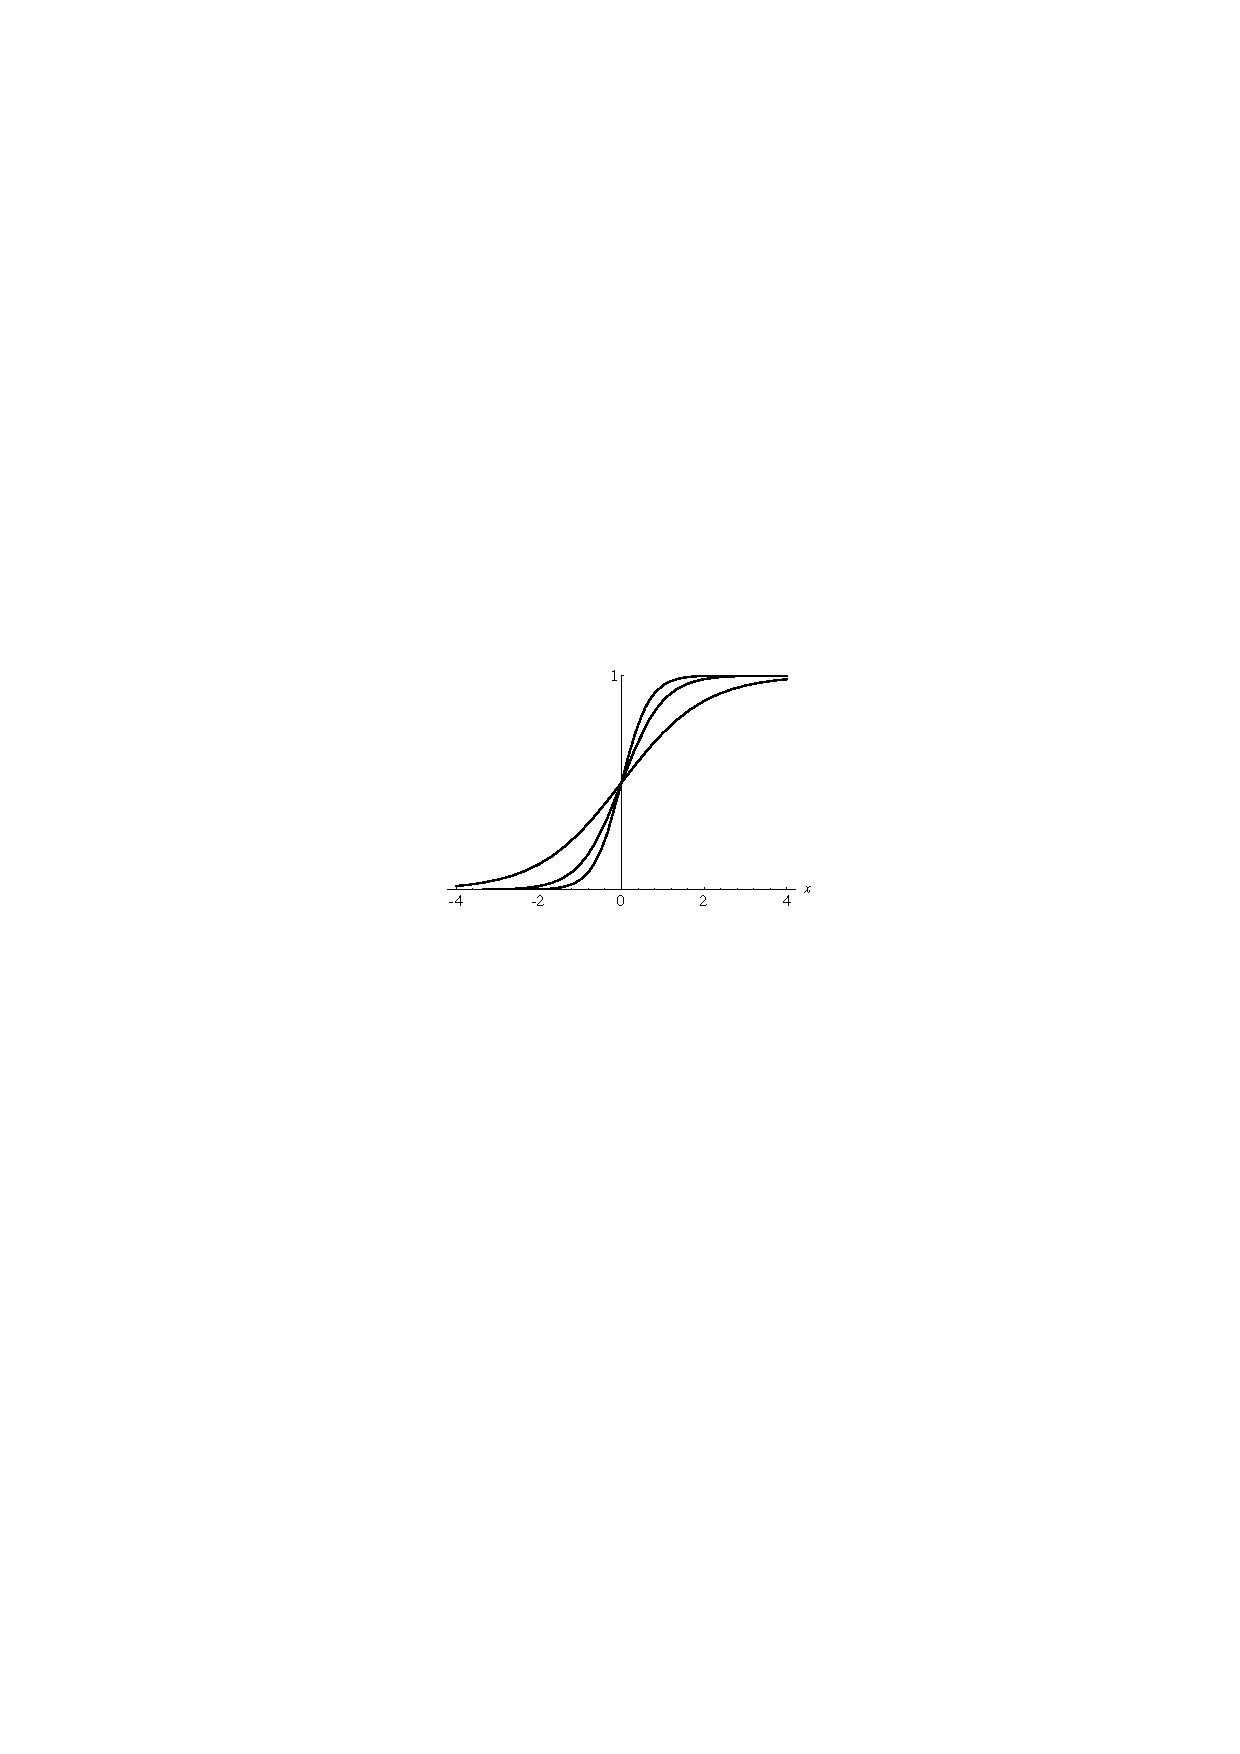
\includegraphics[width=0.7\linewidth]{figures/ch03_sigmoid.pdf}
	\caption{Verlauf der Sigmoid-Aktivierungsfunktion für $c=1$, $c=2$ und $c=3$. Je größer $c$ gewählt wird, desto steiler ist der Anstieg von $0$ auf $1$.}
	\label{fig:ch03_sigmoid}
\end{figure}



% ----------------------------------------------------------------------
% ----------------------------------------------------------------------
\section*{Probleme}
Wie jedes Gradientenverfahren besitzt auch Backpropagation eine Reihe von Problemen, die dadurch entstehen, dass es ein lokales Verfahren ist, welches keine Information über die Fehlerfläche insgesamt hat, sondern nur aus der Kenntnis der lokalen Umgebung (des Gradienten bzw. bei Erweiterungen des Verfahrens zusätzlich einiger vorher besuchter Stellen der Fehlerfläche) ein Minimum suchen muss.

\begin{figure}[ht!] \centering 
	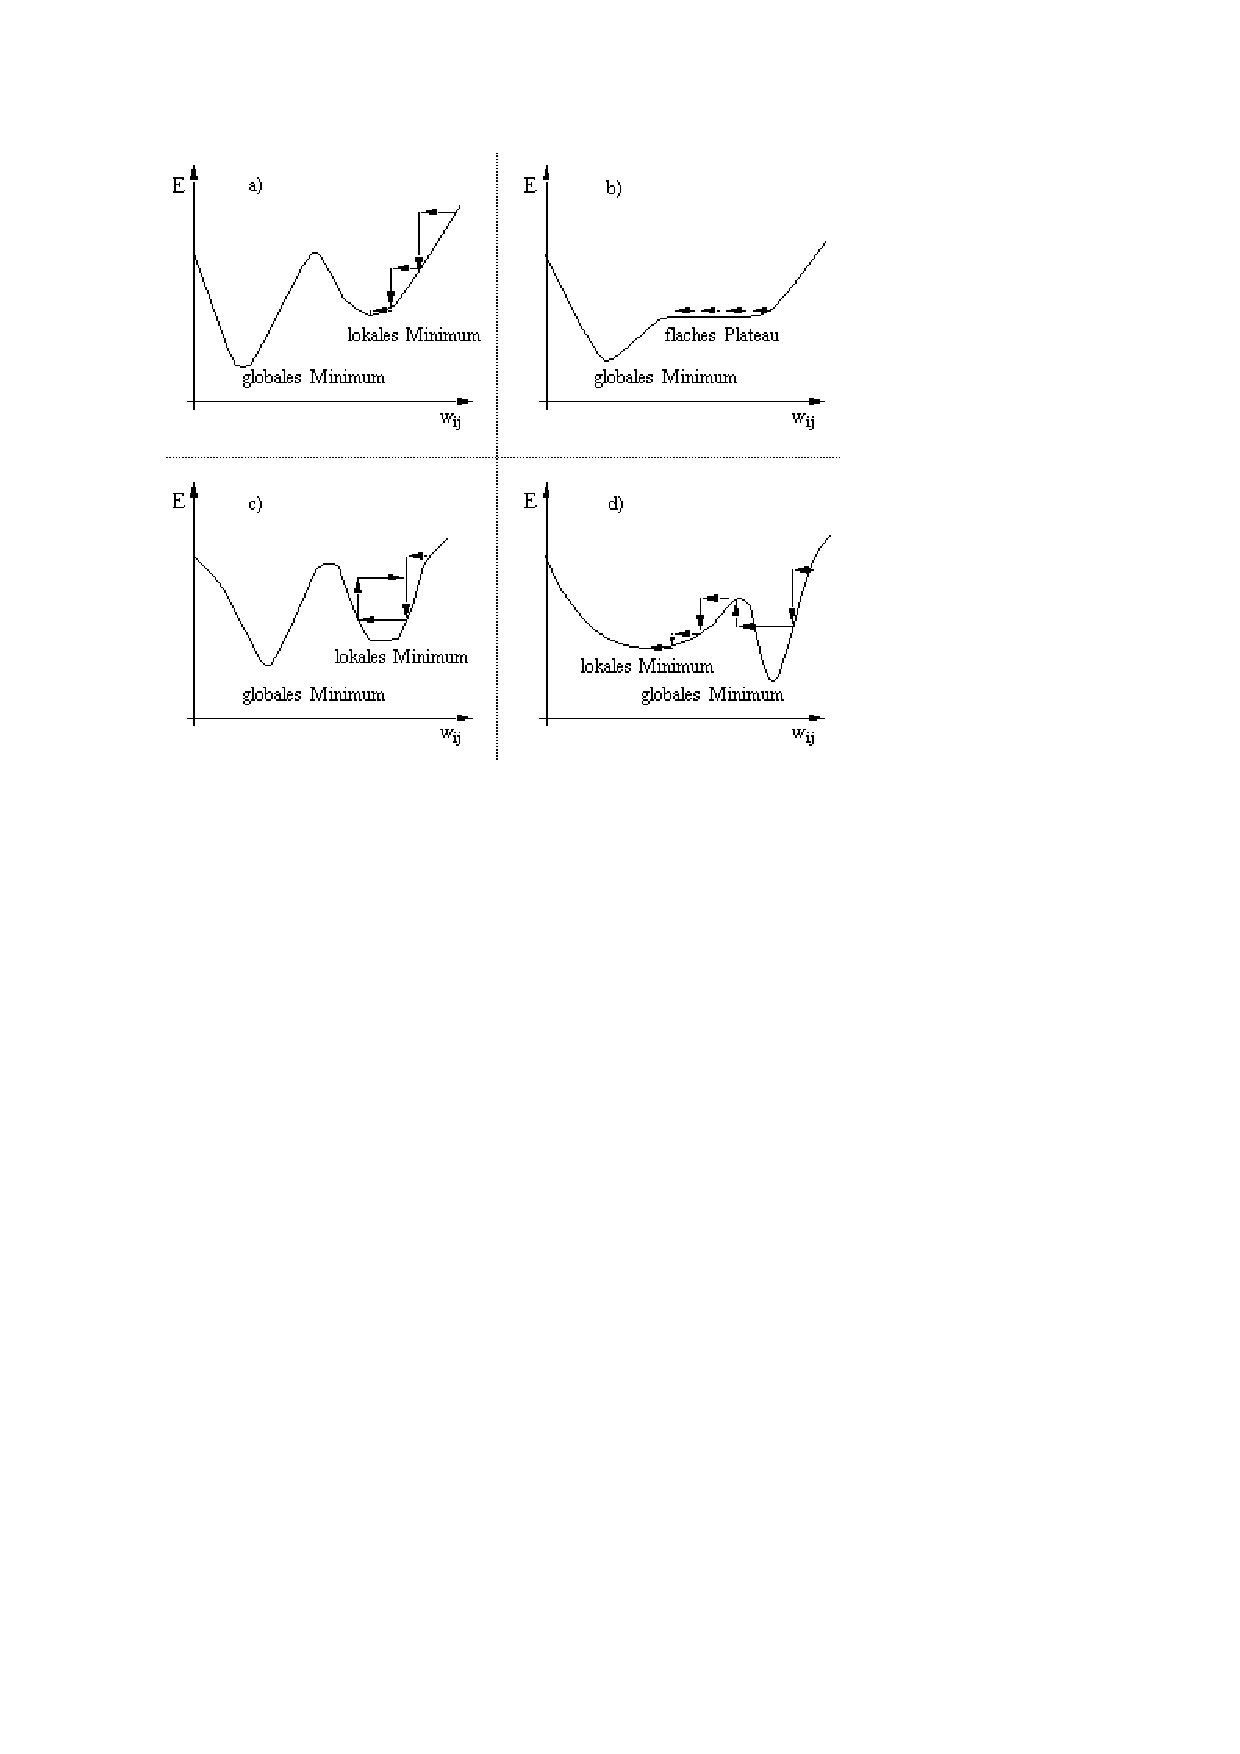
\includegraphics[width=\linewidth]{figures/ch03_fehler-gradientenverfahren.pdf}
	\caption{Problemfälle von Gradientenverfahren: a) lokales Minimum einer Fehlerfläche, b) Fehlerfläche mit Plateau, c) Oszillationen in steilen Schluchten der Fehlerfläche, d) Verlassen guter Minima}
	\label{fig:ch03_sigmoid}
\end{figure}

\subsection*{Lokale Minima der Fehlerfläche}
Gradientenverfahren haben alle das Problem, dass sie in einem lokalen Minimum der Fehlerfläche hängenbleiben können.
Das Problem neuronaler Netze ist, dass die Fehlerfläche mit wachsender Dimension des Netzes (mit wachsender Zahl von Verbindungen) immer stärker zerklüftet wird und daher die Wahrscheinlichkeit, in einem lokalen statt dem globalen Minimum zu landen, immer größer wird.

Zur Lösung solcher Probleme gibt es wenig allgemeingültigen Verfahren, weil sie stark von der Anwendung abhängen.
Die Erfahrung in der Praxis hat jedoch gezeigt, dass Backpropagation bei genügend kleiner Lernrate $\eta$ in sehr vielen Anwendungen ein Minimum findet, das gut genug am globalen Minimum liegt.

\subsection*{Flache Plateaus}
Flache Plateaus der Fehlerfläche sind ein weiteres Problem von Gradientenverfahren. Da die Größe der Gewichtsänderung von dem Betrag des Gradienten abhängig ist, stagniert Backpropagation auf flachen Plateaus, d.h. das Lernverfahren braucht extrem viele Iterationsschritte. 
Handelt es sich um ein vollständig flaches Plateau, ist der Gradient gleich dem Nullvektor und eine Gewichtsänderung findet gar nicht mehr statt.
Einen solchen Stillstand kann man dann nur schwer von dem in einem lokalen oder globalen Minimum unterscheiden, weil auch dort der Gradient ebenfalls der Nullvektor ist.

Für dieses Problem gibt es mit dem \emph{Momentum-Term}, einer Variante von Backpropagation, ein einfaches Verfahren, welches hilft diese Plateaus zu überwinden.

\subsection*{Oszillationen in steilen Schluchten}
In steilen Schluchten der Fehlerfläche kann das Lernverfahren oszillieren. Dies geschieht, wenn der Gradient am Rande einer Schlucht so groß ist, dass durch die Gewichtsänderung ein Sprung auf die gegenüberliegende Seite der Schlucht erfolgt. Ist die Schlucht dort genauso steil, bewirkt dies (da der Gradient jetzt in die andere Richtung zeigt) einen Sprung zurück auf die erste Seite.

Auch hier hilft der Momentum-Term.

\subsection*{Verlassen guter Minima}
Es ist möglich, in der Praxis aber sehr selten, dass Backpropagation aus einem guten Minimum herausspringt, weil der Betrag des Gradienten innerhalb eines sehr engen Tals der Fehlerfläche so groß ist, dass die Gewichtsänderung in ein suboptimales Minimum führt.

Gerade die Verwendung des Momentum-Terms oder die Erhöhung der Lernrate führen zu solchen Problemen.

\subsection*{Wahl der Lernrate}
Die Wahl der Lernrate $\eta$ (Schrittweite) ist entscheidend für das Verhalten des Backpropagation-Algorithmus. Zu große Werte von $\eta$ bewirken starke Sprünge auf der Fehlerfläche und bringen das Risiko mit sich, dass Backpropagation enge Täler nicht findet bzw. dass es aus ihnen wieder herausspringt oder ins Oszillieren gerät.
Zu kleine Werte von $\eta$ bringen einen großen, oft praktisch nicht akzeptierbaren Zeitaufwand für das Training mit sich.

Die Wahl von $\eta$ hängt vom Problem, den Trainingsdaten, sowie der Größe und Topologie des Netzes ab und ist nicht pauschal zu beantworten. Es gibt Verfahren zur Anpassung der Lernrate, welche in einem eigenen Abschnitt erläutert werden.



% ----------------------------------------------------------------------
% ----------------------------------------------------------------------
\section*{Modifikationen von Backpropagation}
\subsection*{Momentum-Term}
Backpropagation mit Momentum-Term (auch konjugierter Gradientenabstieg (engl. conjugate gradient descent)) wurde von Rumelhart, Hinton und Williams beschrieben.
Es ist eine einfache und häufig benutzte Methode zur Vermeidung der Probleme von Backpropagation auf flachen Plateaus und in steilen Schluchten der Fehlerfunktion. 

Die Idee dahinter ist das Einbeziehen der vorangegangenen Gewichtsänderung. Dies führt zu einer \emph{Beschleunigung} (Erhöhung der Gewichtsänderung $\Delta w_{k,h}$) in weiten Plateaus und zu einem \emph{Abbremsen} in stark zerklüfteten Fehlerflächen.

Für die Gewichtsänderung gilt dann:
\[
	\Delta w_{k,h} (t+1) = \eta \cdot o_k \cdot \delta_h + 
		\alpha w_{k,h}(t)
\]

\subsection*{Flat-Spot Elimination}
Ein bekanntes Problem der Backpropagation-Formel ist die Tatsache, dass Neuronen, die im Sättigungsbereich der sigmoiden Aktivierungsfunktion operieren (0 oder 1 bei der logistischen Aktivierungsfunktion), sich nur schwer wieder daraus entfernen, weil ihre Gewichte sich nur um einen minimalen Bruchteil ändern können.

Die Ableitung der Sigmoid-Funktion ist für Neuronen, die stark "`an"' oder "`aus"' sind, d.h. Werte um 0 oder 1 annehmen, nahezu Null. Diese Bereiche, in dem die Ableitung der Aktivierungsfunktion fast Null ist, werden daher \emph{flat spots} genannt (siehe Abbildung \ref{fig:ch03_saettigung-sigmoid-ableitung}.\footnote{Selbst im besten Fall, wenn die Netzeingabe um den Schwellenwert liegt, liefert die Ableitung der Aktivierungsfunktion einen gedämpften Faktor von $0,25$.}

\begin{figure}[ht!] \centering 
	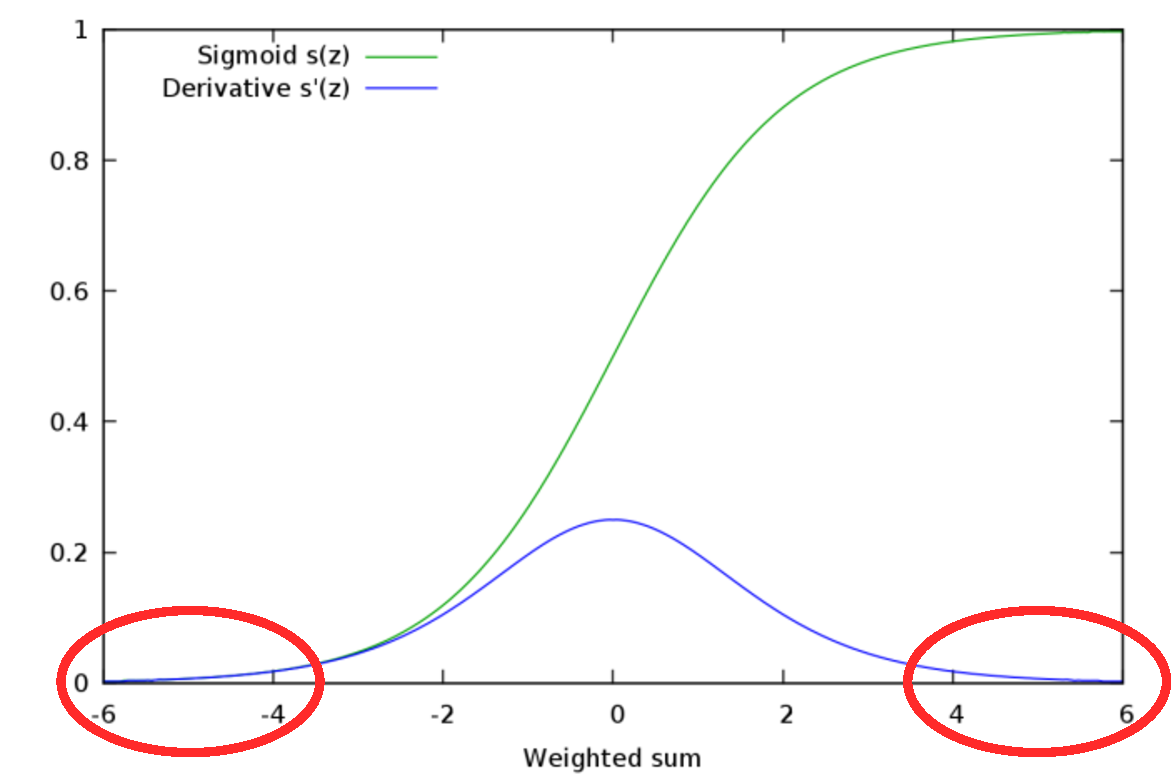
\includegraphics[width=\linewidth]{figures/ch03_saettigung-sigmoid-ableitung.pdf}
	\caption{Ableitung der Sigmoid-Funktion mit Sättigungsbereichen / \emph{flat spots} (gekennzeichnet durch Kreise).}
	\label{fig:ch03_saettigung-sigmoid-ableitung}
\end{figure}

Ein einfache Methode, dieses Problem zu beheben, ist die Anpassung der Ableitung, sodass sie nicht Null wird. Dies ist beispielsweise durch Addition einer Konstanten $0.1$ für alle Werte möglich.
Damit verläuft die Ableitung anstelle von $0$ bis $0.25$ und zurück auf $0$ jetzt von $0.1$ bis $0.35$ und zurück auf $0.1$.
In der Literatur wird diese Variante auch als \emph{modified sigmoid-prime function} bezeichnet.


\subsection*{Manhattan-Training}
% Zell S.103

\subsection*{Quickprop}

\subsection*{Rprop}



